\section{Лекция 2 -- 2024-02-16 -- }
\subsection{Классификация состояний марковской цепи}
\begin{ex}
  Рассмотрим следующую марковскую цепь, которая содержит два состояния:
  \begin{figure}[h!]
    \centering
    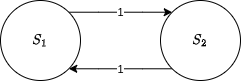
\includegraphics[width=0.3\linewidth]{stoproc/Figures/lec2-ex1}
  \end{figure}
 
  Для неё
  \[
    P = \begin{pmatrix}
      0 & 1 \\
      1 & 0
    \end{pmatrix}, \quad
    P^{2n + 1} = \begin{pmatrix}
      0 & 1 \\
      1 & 0
    \end{pmatrix}, \quad
    P^{2n} = \begin{pmatrix}
      1 & 0 \\
      0 & 1
    \end{pmatrix}.
  \]
  Очевидно, такая последовательность не может иметь предела, поэтому такая марковская цепь не
  эргодичная.

  Однако в этой марковской цепи существует стационарное распределение, поскольку СЛАУ
  $\bm\pi^T = \bm\pi^{\mathsf T} P;\ \sum \pi_j = 1$ даёт решение
  $\bm\pi^{\mathsf T} = (0.5, 0.5)$.
\end{ex}

\begin{ex}
  Рассмотрим марковскую цепь, содержащую состояния некоторого устройства. Пусть первое 
  состояние соответствует работоспособности устройства, второе и третье
  соответствуют небольшой поломке (возможен ремонт),
  четвертое --- устройство сломано полностью (такое устройство списывают).
  \begin{figure}[h!]
    \centering
    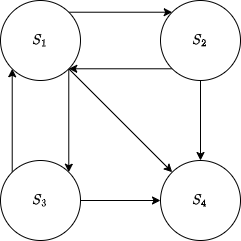
\includegraphics[width=0.3\linewidth]{stoproc/Figures/lec2-ex2}
  \end{figure}
  
  Стрелками на рисунке помечены ненулевые вероятности (для примера неважны их
  значения).
  \[
    P = \begin{pmatrix}
      \cdots & \cdots & \cdots & \cdots\\
      \cdots & \cdots & \cdots & \cdots\\
      \cdots & \cdots & \cdots & \cdots \\
      0 & 0 & 0 & 1
    \end{pmatrix}.
  \]
  И тогда $\mathbf p = (0, 0, 0, 1)$ является стационарным распределением.
  Интуитивно также понятно, что прибор, начиная с любого состояния, рано или поздно сломаемся.
  Таким образом, данная марковская цепь не является эргодической.
\end{ex}

\begin{ex}
  Рассмотрим марковскую цепь
  \begin{figure}[h!]
    \centering
    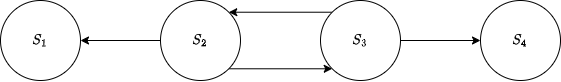
\includegraphics[width=0.7\linewidth]{stoproc/Figures/lec2-ex3}
  \end{figure}
  
  Для неё стационарными распределениями будут являться $(1, 0, 0, 0)$
  и $(0, 0, 0, 1)$. Она тоже не является эргодической, так как нет финальных
  вероятностей.
\end{ex}

\begin{definition}
  Состояние $S_i$ (или множество состояний) называется \emph{несущественным}, если
  существуют $ S_j $ и $ n\in \mathbb N $, для которых $p_{ij}^{(n)} > 0$, --- из
  этого состояния можно выйти ---
  но для всякого $ S_k $ и $ m \in \mathbb N $ выполняется $p_{ki}^{(m)} = 0$ --- в это состояние нельзя попасть.
\end{definition}

\begin{definition}
  Состояние (или множество состояний) называется \emph{поглощающим}, если в него
  можно войти ---
  $\exists S_j , \exists n\colon p_{ji}^{(n)} > 0$,
  но нельзя выйти ---
  $\forall S_j, \forall n \colon p_{ij}^{(n)} = 0$.
\end{definition}

\begin{definition}
  Говорят, что состояние $S_i$ \emph{достижимо} из состояния $S_j$, если $\exists n\colon p_{ji}^{(n)} > 0$.
\end{definition}

\begin{definition}
  Если $S_i$ достижимо из $S_j$, $S_j$ достижимо из $S_i$, то $S_i$ и $S_j$
  называют \emph{сообщающимеся
  состояниями}.
\end{definition}

Отношение сообщаемости является рефлексивным, транзитивным и симметричным, поэтому оно является 
отношением эквивалентности, то есть отношение сообщаемости разбивает марковскую цепь на классы эквивалентности.

\begin{definition}
  Если марковская цепь состоит из одного класса эквивалентности, то она называется
  \emph{неразложимой}.
\end{definition}

\begin{ex}\label{ex:724}
  Для марковской цепи с графом, изображённым на рисунке \ref{fig:ex4},
  \begin{figure}[h!]
    \centering
    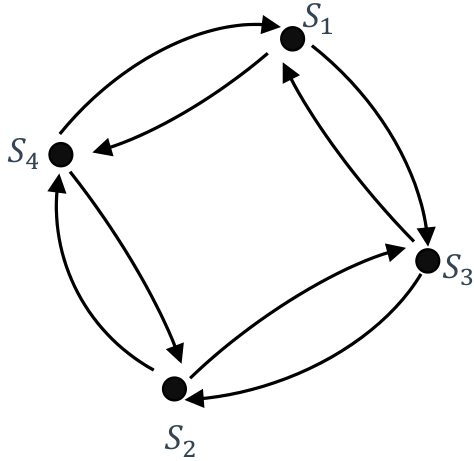
\includegraphics[width=0.3\textwidth]{stoproc/Figures/lec2-ex4.png}
    \caption{Граф цепи примера \ref{ex:724}.}
    \label{fig:ex4}
  \end{figure}
  \[
    P = \begin{pmatrix}
      0 & 0 & 1/2 & 1/2 \\
      0 & 0 & 1/2 & 1/2 \\
      1/2 & 1/2 & 0 & 0 \\
      1/2 & 1/2 & 0 & 0
    \end{pmatrix}, \quad
    P^2 = \begin{pmatrix}
      1/2 & 1/2 & 0 & 0 \\
      1/2 & 1/2 & 0 & 0 \\
      0 & 0 & 1/2 & 1/2 \\
      0 & 0 & 1/2 & 1/2
    \end{pmatrix}.
  \]

  То есть начиная в $S_1$ или $S_2$, попадем в $S_3$ или $S_4$, а потом назад в $S_1$, $S_2$.
Такая ситуация называется \emph{цикличностью}.
\end{ex}

\begin{definition}
  Говорят, что состояние $S_i$ \emph{имеет период $d(i) = d$}, если
  \begin{enumerate}
    \item Из $p_{ii}^{(n)} > 0$ вытекает $n = d \cdot l,\ l \in \mathbb{N}$ ($n$ делится на $d$).
    \item Число $d$ есть наибольший общий делитель всех таких $n$, для которых
      выполнено первое условие.
  \end{enumerate}
\end{definition}
Например, в задаче \ref{ex:724} период $d(1, 2, 3, 4) = 2$.

\begin{definition}
  Если $d(i) = 1$, то состояние называется \emph{апериодическим}.
  Если $p_{ii}^{(n)} = 0$ для всех $n$, то считают $d(i) = 0$.
\end{definition}

% Следующая теорема есть в Ширяеве
\begin{theorem}
  Если $\mathscr S = \left\{ S_1, \dots, S_n \right\} $, марковская цепь неразложима и все состояния
  периодические, то $d(i) = d(j)$ для всех $ i $, $ j $.
\end{theorem}
\begin{proof}
  Выберем $S_i$ периодическим с периодом $d(i)$, а $S_j$ --- с периодом $d(j)$.
  Необходимо доказать, что $d(i) = d(j)$.
  \begin{multline*}
    \begin{cases}
    \exists k : p_{ij}^{(k)} > 0, \\
      \exists l : p_{ji}^{(l)} > 0
    \end{cases}
    \Rightarrow \text{по т-ме Колмогорова-Чепмена: } \\
    p_{ii}^{(k+l)} = \sum_{\alpha} p_{i\alpha}^{(k)} \cdot p_{\alpha i}^{(l)} 
    \geqslant p_{ij}^{(k)} \cdot p_{ji}^{(l)} > 0
    \Rightarrow
    k+l \text{ делится на $d(i)$}.
  \end{multline*}
  если $n$ не делится на $d(i)$, то $n+k+l$ не делится на $d(i)$, тогда $p_{ii}^{(n+k+l)} = 0$, 
  тогда $p_{ii}^{(n+k+l)} = \sum_{\alpha} \sum_\beta p_{i\alpha}^{(k)} p_{\alpha \beta}^{(n)} 
  p_{\beta i}^{(l)}$, тогда $p_{jj}^{(n)} = 0$ тогда $n$ не делится на $d(j)$.

  если $p_{jj}^{(n)} > 0 \Rightarrow$ $n$ делится на $d(i)$, а по предположению теоремы $n$ делится 
  на $d(j)$ $\Rightarrow$ $d(i) \leqslant d(j)$.

  Аналогично можно доказать, что $d(j) \leqslant d(i)$. То есть $d(i) = d(j)$.
\end{proof}

\begin{definition}
  Этот общий период называется периодом цепи $d(S)$.
  Если $d(S) = 1$, то цепь называется апериодической -- все состояния непериодические.
\end{definition}

\begin{theorem}
  Марковская цепь с конечным множеством состояний является эргодической тогда и только тогда,
  когда она апериодична и неразложима.
\end{theorem}
(\emph{Без доказательства.})

\begin{theorem}
  Марковская цепь со счетным множеством состояний является эргодической тогда и только тогда,
  когда она неразложима, апериодична, возвратна и положительна.
\end{theorem}
(\emph{Без доказательства.})

\begin{definition}
  Состояние $S_i$ называется \emph{возвратным}, если $\sum\limits_{n=1}^{\infty} f_{ii}^{(n)} = 1$,
  где 
  \[
    f_{ii}^{(n)} = P(\xi_n = i, \xi_{n-1} \neq i, \dots, \xi_1 = i \mid \xi_0 = i).
  \]
\end{definition}

\begin{definition}
  Цепь называется \emph{возвратной}, если все ее состояния возвратны.
\end{definition}

\begin{definition}
  Состояние $S_i$ называется \emph{положительным}, если
  $\sum\limits_{n=1}^{\infty} n f_{ii}^{(n)} < \infty$.
  (Математическое ожидание конечно, то есть можем вернуться за конечное число шагов.)
\end{definition}

\begin{definition}
  Цепь называется \emph{положительной}, если все ее состояния положительны.
\end{definition}


\begin{ex}
  % TODO рисунок бесконечная гусеница
  $p+q=1$.

  \[
    P = \begin{pmatrix}
      0 & 1 & 0 & \dots \\
      q & 0 & p & \dots \\
      0 & q & 0 & p \\
      \vdots & \vdots & \vdots & \vdots
    \end{pmatrix} 
  \]

  Найдём стационарные состояния:
  \[
    \bm\pi^{\mathsf T} = \bm\pi^{\mathsf T} P \Leftrightarrow
    \begin{cases}
      \pi_0 = q \pi_1, \\
      \pi_1 = \pi_0 + q \pi_2, \\
      \dots, \\
      \pi_k = p \pi_{k-1} + q \pi_{k+1}.
    \end{cases}
  \]
  Получили рекуррентное уравнение. Применим алгоритм его решения.
  Характеристическое уравнение имеет вид $q \lambda^2 - \lambda + p = 0$ с
  корнями
  \[
    \lambda_{1, 2} = \dfrac{1\pm \sqrt{1-4pq}}{2q} = \dfrac{1 \pm \sqrt{1 - 4(1-q)q}}{2q}
    = \dfrac{1 \pm |1 - 2q|}{2q}.
  \]
  \begin{enumerate}
    \item $q > \dfrac{1}{2}$ -- движение влево более вероятно, чем вправо.
      \[
        \lambda_{1, 2} = 1, \dfrac{1-q}{q}.
      \]
      $\pi_k = c_1 \cdot 1^k + c_2 \cdot \left( \dfrac{p}{q} \right)^k$.
      Причем $0 < \pi_k < 1$ $\Rightarrow$ и $\sum_{k=0}^\infty \pi_k = 1$.
      Получаем, $C_1 = 0, \sum_{k=0}^\infty C_2 \left( \dfrac{p}{q} \right)^k 
      \Rightarrow C_2 = \dots = \dfrac{q-p}{q}$
      % TODO дописать из семинара

      Получили эргодичность.

    \item $q = \dfrac{1}{2}$ тогда $\lambda_{12} = 1$ -- двукратный корень. $\pi_k = C_1 + C_2 k$. 
      Тогда $\pi_k = 0$, а цепь неэргодичная.

    \item $q<\dfrac{1}{2}$. $\lambda_{1, 2} = \dfrac{1 \pm (1-2q)}{2q} = \dfrac{p}{q}, 1$.
      $\pi_k = C_1 + C_2 \left(\dfrac{p}{q}\right)^{k} \Rightarrow \pi_k = 0$.
  \end{enumerate}
\end{ex}

\begin{definition}
  Пусть конечное множество состояний $\mathscr S = \left\{ S_1, \dots, S_m \right\} $. Берём подмножество 
  состояний (для определенности первые $m_1 < m$ состояний)
  $A = \left\{ S_1, \dots, S_{m_1} \right\} $.
  Обозначим $H^A = \inf \left\{ n\geqslant 0,\, \xi_n \in A \right\} $ --- момент первого достижения 
  множества $A$.
  Обозначим $h^A = P(H^A < \infty \mid \xi_0 = i)$,
  $\mu^A_i = M(H^A \mid \xi_0 = i)$.
\end{definition}

\begin{theorem}
  Если $A \subset \mathscr S$, то $h_i^A$ --- наименьшее неотрицательное решение системы
  \[
    h^A_i = \begin{cases}
      1, & S_i \in A, \\
      \sum_{j=1}^m p_{ij} h_j^A, &S_i \notin A.
    \end{cases}
  \]
  $\mu^A_i = 0, S_i \in A$
  $\mu^A_i = 1 + \sum_{j=m_1+1}^{m} p_{ij} \mu_j^A, S_i \notin A$.
\end{theorem}
